\documentclass{article}
\usepackage[T2A]{fontenc}
\usepackage[utf8]{inputenc}
\usepackage[russian]{babel}
\usepackage[margin=1.5cm]{geometry}
\usepackage{icomma}
\usepackage{amsmath}
\usepackage{amssymb}
\usepackage{enumitem}
\usepackage{graphicx}
\usepackage{url}
\usepackage{xfrac}
\usepackage{fancyvrb}

\pagestyle{empty}


\begin{document}

% ==============================================================================

\begin{flushright}
    \textit{Выполнил: Максимов Н. Д.} \\
    \textit{Группа: 09-414} \\
    \textit{Вариант: 8}
\end{flushright}

\begin{center}
    \bfseries\LARGE Отчет по лабораторной работе №4
\end{center}
\bigskip

% ==============================================================================

\subsection*{Постановка задачи}

В соответствии с заданием необходимо, используя две данные выборки $X$ и $Y$, решить следующие задачи:

\begin{enumerate}
    \item Построить уравнение линейной регрессии $X$ по $Y$ $\hat x = ay + b$, где коэффициенты $b$ и $a$ вычисляются по формулам:
    \[ a = \frac{\overline{xy} - \overline x \cdot \overline y}{\overline{y^2} - \overline y ^ 2} \qquad\qquad b = \overline x - a \overline y \]
    \item Вычислить выборочный коэффициент корреляции по формуле:
    \[ \hat r = \frac{\overline{xy} - \overline x \cdot \overline y}{S_x \cdot S_y}, \]
    где $S_x$ и $S_y$ стандартные отклонения выборок $X$ и $Y$ соответственно.
    \item Выполнить прогноз $x$ по значению $y=79$.
\end{enumerate}

% ==============================================================================

\subsection*{Полученные значения}

\paragraph{Выборочный коэффициент корреляции} $\hat r = 0.4325$ \\
Значение находится в интервале от 0.3 до 0.5, что говорит об умеренной (слабой) положительной линейной связи между выборками.

\paragraph{Уравнение линейной регрессии} $\hat x = 0.57y + 72.06$

\paragraph{Прогноз значения} Расчетное (спрогнозированное) значение $x=116.92$ при заданном $y = 79$.

\begin{center}
    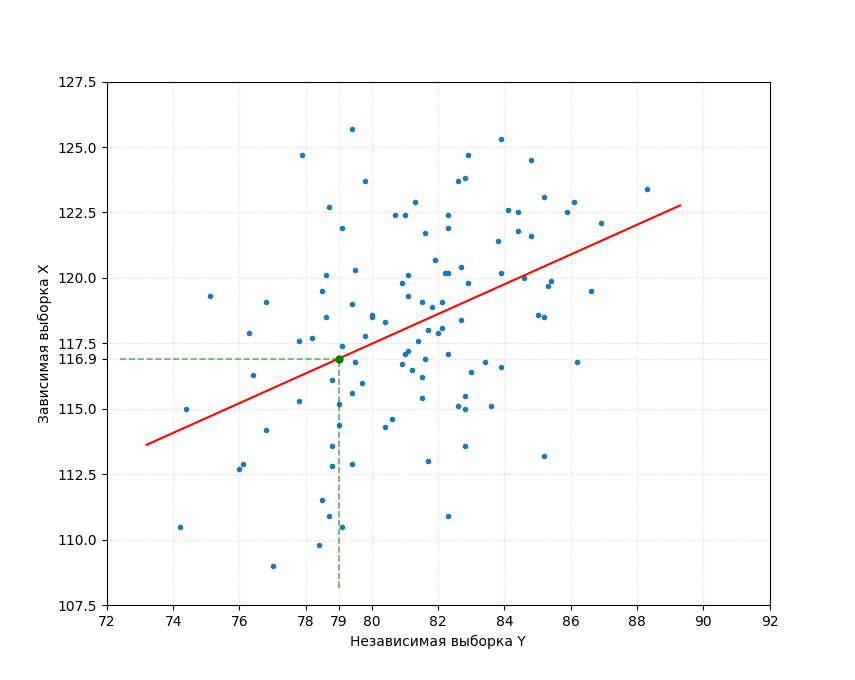
\includegraphics[width=0.75\textwidth]{picture.png}
\end{center}

% ==============================================================================

\subsection*{Листинг}

\noindent \texttt{statools.py}
\VerbatimInput[tabsize=4, fontsize=\small, numbers=left]{../source/statools.py}
\noindent \texttt{main.py}
\VerbatimInput[tabsize=4, fontsize=\small, numbers=left]{../source/main.py}

% ==============================================================================

\vfill
\bigskip
\noindent\rule{\textwidth}{0.4pt}
\small Полный исходный код лабораторной работы доступен в репозитории на GitHub: \url{https://github.com/mndkpfu/MS}

\end{document}